\documentclass[11pt]{article}
\usepackage{graphicx}
\begin{document}

\begin{titlepage}

\begin{center}
\begin{huge}
Swarm Visualiser - COS 301 Main Project
\\
Design Specification- General Purpose Optimiser
\begin{small}
\\
Team: Dragon Brain
\\
Members:
\\
Matheu Botha u14284104
\\
Renton McInytre u14312710
\\
Emilio Singh u14006512
\\
Gerard van Wyk u14101263

\end{small}

\end{huge}
\end{center}
\end{titlepage}

\pagebreak

\tableofcontents
\pagebreak
\section{System Component: General Optimiser}
\subsection{Purpose}
\paragraph{}
The SwarmVis program is comprised of many separate parts. Crucial to the point of the visualisation, is the actual optimiser whose results need to be visualised. This is a service performed by the OPT Module which is described in this text.
\subsection{Relation to System as a Whole}
\paragraph{}
The OPT module will perform whatever optimisation task it has been configured to do and then place its results, as they happen, into the Model component of the system. From there, the Graphical Pipeline will be responsible for rendering the results to the screen. The OPT module is largely independent of the other modules and the other modules, especially, are independent of it. The only interaction that occurs between the OPT module and the rest of the system is the user configuration mediated by the interface and the message passing from the OPT module to the Model module.

\section{Processes and Requirements}
\paragraph{}
This section will detail the various ways in which the OPT module will interact with external components. This is divided roughly into Configuration Requirements and Message Passing. This is by no means the length and breadth of the scope of the module but rather the most apparent requirements for consideration.

\subsection{Configuration Requirements}
The OPT needs to be configurable in terms of allowing some external user to change operational parameters such that the OPT, for that run, will behave differently.

To that end, the following are areas for consideration for external configuration requirements:

\begin{itemize}
\item Size of the Swarm
\item Initial Placement of particles by the user
\item Random Placement of particles as chosen by user
\item Which Optimisation method to use: Hill Climbing, Random Search or PSO(and variants)
\item Which Objective Function to use
\item If the system should favour the Cognition or Social component when using PSO
\item The Dimensions of the problem space in terms of:
	\begin{itemize}
	\item The number of dimensions
	\item The upper and lower bounds of each dimension
	\end{itemize}
\item Whether the system should halt prematurely or not	
\end{itemize}

\subsection{Message Passing}
\paragraph{}
A requirement of the MVC pattern is that we require the use of a Model. The Model will be our common data storage and organisational area whose purpose will be to receive progress updates about how the optimisation process is going based on the real-time results of the optimiser and then to be capable of sending those results to the graphics pipeline for processing. \\ It is therefore crucial that the Model be able to receive updates from the Optimisation module in a format it can understand and efficiently process.

\section{Proposal for Additional Component}
One of the added levels of functionality expressed by the client was the use of multiple optimisers functioning on screen at the same time. In order to achieve this, a high level controller module, called an Overseer, could be implemented such that it would be able to create and control OPT modules and then use concurrent threading to concurrently process all optimisation at once.

This would naturally increase the system's computational and memory requirements by a significant factor. Additionally, it would require a highly adaptive Model component that could create separate but concurrent storage for optimisation updates and still provision them to the Graphics Pipeline without significant delays. This is a contentious topic and will further discussion.

\section{Class Diagram of Component}

\begin{figure}
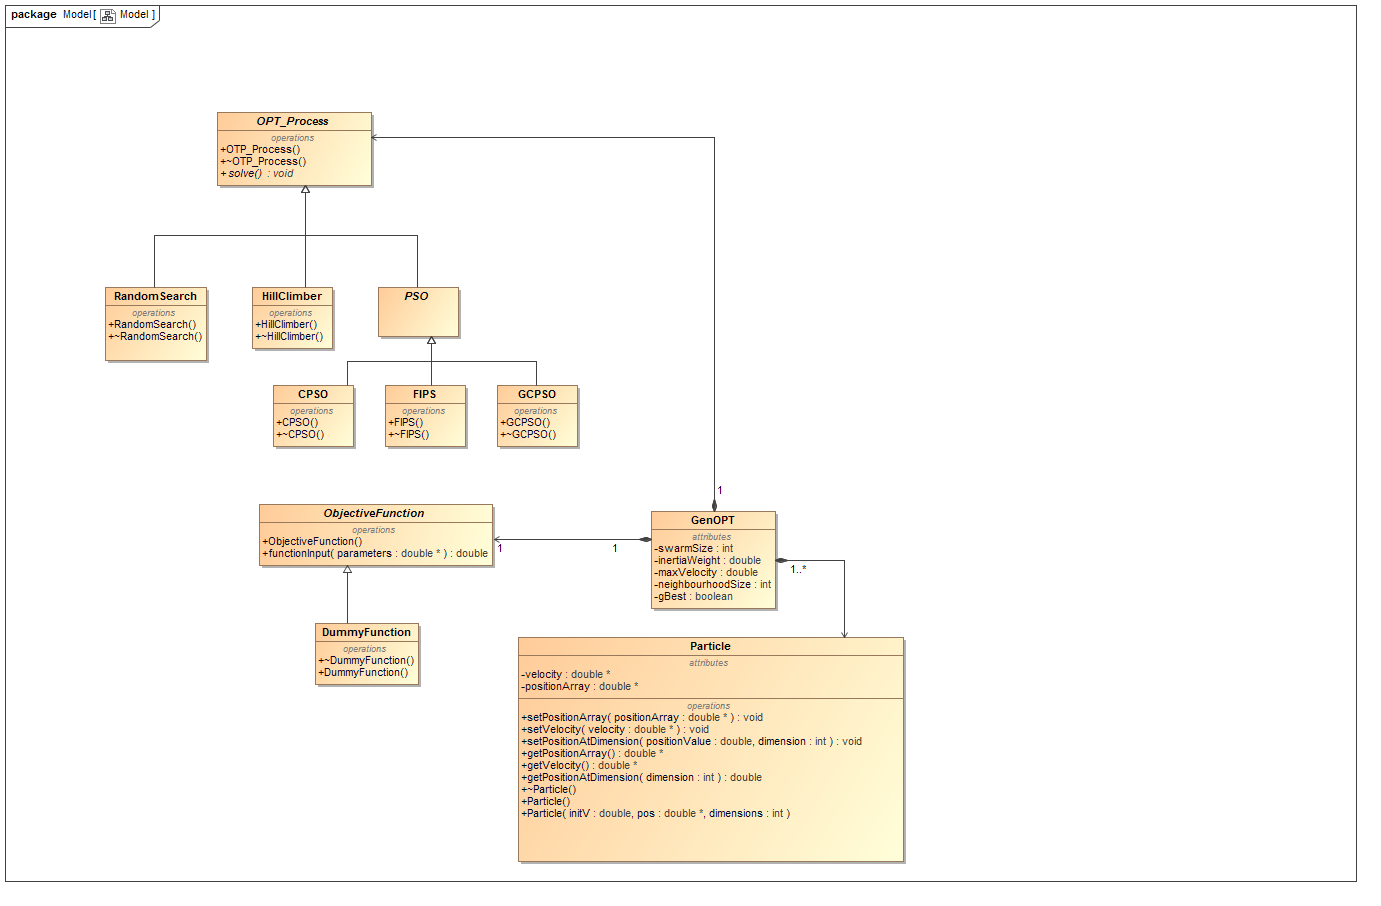
\includegraphics[scale=0.38]{Model.png}
\caption{The diagram presented above is the class diagram explaining the structure of the OPT Module}
\end{figure}

\end{document}
